\documentclass[../../General.tex]{subfiles}
\begin{document}


%----------------------------------------------------------------------------------------
%	LAZOS DE CONTROL
%----------------------------------------------------------------------------------------

\section{Lazos de control}\label{sec:lazos_control}

El robot regula cuatro magnitudes: la velocidad de cada rueda posterior, el ángulo de dirección de las ruedas frontales, la altura del plano óptico del piranómetro y la inclinación de la plataforma que lo porta. Los lazos se reparten entre los dos niveles de procesamiento definidos en la Sección \ref{subsec:interconexion_serial} y en la arquitectura del Capítulo 6. La Raspberry Pi 4 ejecuta el seguimiento de la ruta y fija las consignas de velocidad, de dirección, de altura y de inclinación. El Arduino Mega 2560 Pro cierra los lazos de velocidad de las ruedas, genera los pulsos de los motores paso a paso y de los servomotores, lee los sensores inerciales y aplica las protecciones de los actuadores. Las lecturas del microcontrolador llegan a la computadora en la trama de $50\text{ tramas/s}$ descrita en la Sección \ref{subsec:interconexion_serial}.
% PENDIENTE: la Sección subsec:interconexion_serial describe solo la trama del microcontrolador hacia la computadora; falta definir la trama de consignas de la computadora hacia el microcontrolador (velocidad, dirección, altura, inclinación y habilitaciones).

La medición de irradiancia se realiza con el robot detenido y solo en tramos casi planos (Secciones \ref{sec:subsistema_orientacion} y \ref{sec:subsistema_elevacion}). Por ello, los lazos de altura y de inclinación actúan con el vehículo parado, y el lazo de traslación actúa con el mecanismo de elevación en su posición inferior en los desplazamientos largos.

%----------------------------------------------------------------------------------------

\subsection{Lazo de traslación y dirección}\label{subsec:lazo_traslacion}

El vehículo avanza con tracción en el eje posterior, con un motorreductor por rueda, y vira con una dirección Ackermann en el eje frontal accionada por dos servomotores (Sección \ref{sec:subsistema_traccion}). El control de la traslación tiene dos niveles, como se observa en la Figura \ref{fig:LazoControl}.

\subsubsection{Seguimiento de la ruta}

En la computadora, la posición del robot se obtiene del receptor GNSS SAM-M8Q, el rumbo de la guiñada que entrega el BNO055 y el avance medido por los encoders de las ruedas posteriores. Con esa estimación, el algoritmo Pure Pursuit, seleccionado en la matriz morfológica, busca sobre la ruta el punto situado a una distancia de anticipación $l_d$ del eje posterior y calcula el arco que une ambos puntos. Si $\alpha$ es el ángulo entre el rumbo del robot y la recta hacia ese punto, la curvatura del arco y el ángulo de dirección equivalente en el centro del eje frontal son:
% PENDIENTE: citar la fuente del algoritmo Pure Pursuit (por ejemplo, Coulter, 1992, CMU-RI-TR-92-01); no está en biblio.bib y el usuario debe añadirla a Referencias.
% PENDIENTE: la distancia de anticipación l_d no está definida.
% PENDIENTE: la exactitud de posición del SAM-M8Q no está declarada en el Capítulo 6; verificar si basta para seguir un pasillo.
% PENDIENTE: el método de fusión de GNSS, BNO055 y odometría no está definido.

\begin{equation}\label{eq:pure_pursuit}
    \kappa = \frac{2\sin\alpha}{l_d}, \qquad \delta = \arctan\left(L\,\kappa\right)
\end{equation}

donde $L$ es la distancia entre ejes. La relación $\tan\delta = L/R$ es la misma del modelo cinemático de la Sección \ref{sec:subsistema_traccion} \citep{siegwart2004mobile, jazar2017vehicle}, con $R = 1/\kappa$. El ángulo $\delta$ se limita al que corresponde al radio mínimo de giro $R_{\min}$ del subsistema de tracción y dirección, es decir, a $\arctan\left(L/R_{\min}\right)$.

La consigna de velocidad de avance es la velocidad nominal de $1.0\text{ m/s}$ del requerimiento 3 (Tabla \ref{tab:lista_requerimientos}) y pasa a cero en cada punto de medición.

\subsubsection{Dirección}

El microcontrolador convierte el ángulo $\delta$ en los ángulos de la rueda interior y exterior con la condición de Ackermann \citep{siegwart2004mobile, jazar2017vehicle}:

\begin{equation}\label{eq:ackermann_control}
    \delta_i = \arctan \left[ \frac{L}{R - \frac{b}{2}} \right], \qquad \delta_o = \arctan \left[ \frac{L}{R + \frac{b}{2}} \right]
\end{equation}

donde $b$ es la distancia entre los pivotes. Cada ángulo se envía a su servomotor como un pulso de $500$ a $2500\text{ }\mu\text{s}$ cada $20\text{ ms}$, con la posición de avance en línea recta en $1500\text{ }\mu\text{s}$ (Capítulo 6). Cada servomotor cierra su propio lazo de posición con su potenciómetro interno, de modo que, desde el microcontrolador, la dirección se comanda en lazo abierto.
% PENDIENTE: relación entre el ancho de pulso y el ángulo de cada mangueta (calibración del servomotor montado).

\subsubsection{Velocidad de las ruedas posteriores}

Para que las ruedas posteriores no se arrastren en los virajes, el diferencial electrónico fija una consigna de velocidad angular para cada rueda a partir de la velocidad de avance $v$, del radio de la rueda $r$ y del radio de giro $R$ \citep{siegwart2004mobile, jazar2017vehicle}:

\begin{equation}\label{eq:diferencial_control}
    \omega_{r,i}^{*} = \frac{v}{r} \left[ 1 - \frac{b}{2R} \right], \qquad \omega_{r,o}^{*} = \frac{v}{r} \left[ 1 + \frac{b}{2R} \right]
\end{equation}

Cada rueda tiene su propio lazo cerrado de velocidad con un controlador PID, seleccionado en la matriz morfológica. La realimentación es el encoder E6B2-CWZ6C de la rueda, decodificado en modo $2\times$, con $2000$ cuentas por revolución (Sección \ref{subsec:encoder}). La salida del controlador es el ciclo de trabajo de las entradas PWMA y PWMB del controlador de puente H, a $20\text{ kHz}$: para avanzar se modula PWMA con PWMB en nivel bajo, y para retroceder, a la inversa \citep{pololu_h2_36v11}.
% PENDIENTE: ganancias del PID y período de muestreo del lazo de velocidad.

El ciclo de trabajo que entrega el PID queda sujeto a las limitaciones definidas en el Capítulo 6:
\begin{itemize}
    \item se limita a $24\text{ V}/V_{\text{bat}}$, con la tensión que mide el monitor LTC2944, porque los motores son de $24\text{ V}$ y la batería llega a $29.4\text{ V}$;
    \item se reduce cuando la corriente medida en la salida CS supera $8\text{ A}$;
    \item la tracción se corta si la rueda no gira, según su encoder, mientras el ciclo de trabajo es mayor que cero;
    \item si una salida FLT pasa a nivel bajo, el controlador quedó enclavado por una falla y se reinicia con la salida común conectada a las entradas SLP.
\end{itemize}
Como cada rueda tiene su encoder, la comparación de ambas lecturas con la relación de la Ecuación \ref{eq:diferencial_control} permite además detectar el deslizamiento de una rueda (Sección \ref{subsec:encoder}).

\begin{figure}[H]
	\captionsetup{justification=raggedright, singlelinecheck=false, labelsep=none}
	\caption[Lazo de control de traslación y dirección.]{}
	\textit{Lazo de control de traslación y dirección.} \par\medskip
	\centering
	% PENDIENTE: regenerar la figura (la actual muestra tracción diferencial). Bloques: ruta (microSD) -> Pure Pursuit (Raspberry Pi) -> delta -> Ackermann -> delta_i, delta_o -> servomotores M3, M4 (lazo interno); delta y v* -> diferencial electrónico -> omega* izquierda y derecha -> PID (Arduino) -> limitador de ciclo de trabajo (24 V/V_bat, 8 A) -> puente H -> motorreductor M5, M6 -> rueda; realimentación por encoder a cada PID; GNSS, BNO055 y odometría -> estimación de posición y rumbo -> Pure Pursuit. Renombrar el archivo sin tilde.
	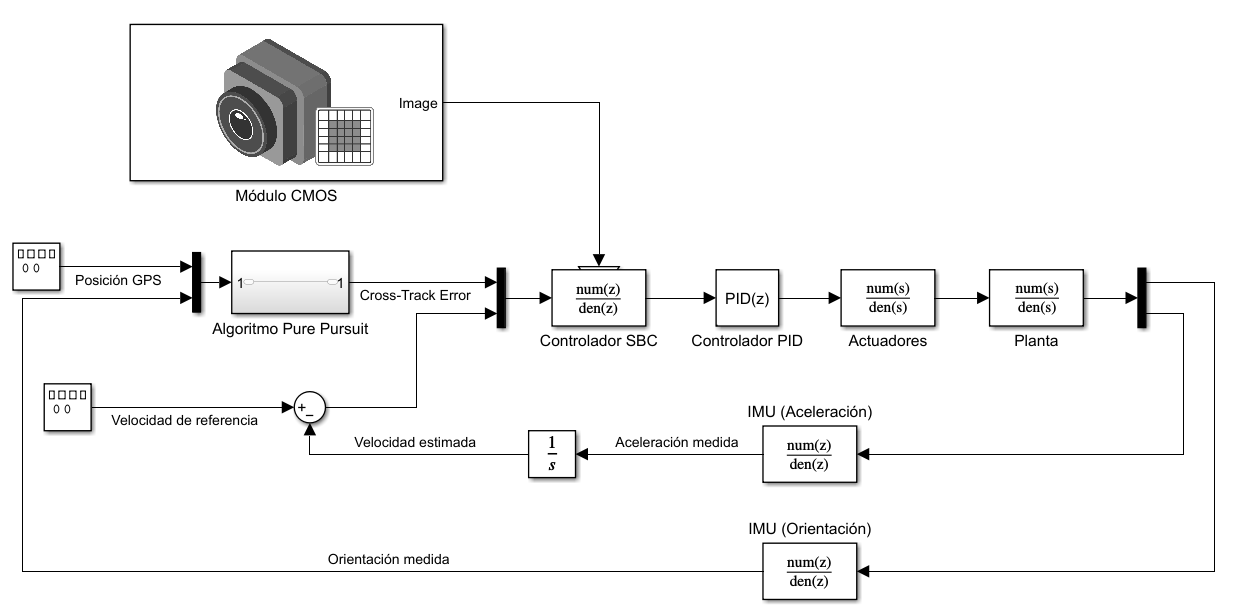
\includegraphics[width=\textwidth]{Recursos/Imagenes/ImagenesDisenoProgramacion/LazoControlNavegación.png} \par\medskip
	\raggedright
	\footnotesize \textit{Nota.} Elaboración propia.
	\label{fig:LazoControl}
\end{figure}

%----------------------------------------------------------------------------------------

\subsection{Lazo de altura del plano óptico}\label{subsec:lazo_altura}

La altura del plano óptico se ajusta con el robot detenido. La consigna es una altura $H^{*}$, que se convierte en el ángulo de los brazos invirtiendo la Ecuación \ref{eq:altura_elev}:

\begin{equation}\label{eq:consigna_altura}
    \theta^{*} = \arcsin\left( \frac{H^{*} - z_p - A - z_c}{L} \right)
\end{equation}

y se acota al rango de operación de $15^\circ$ a $70.31^\circ$ del mecanismo. La realimentación es el ángulo del brazo inferior medido por su MPU-6050. Como este sensor mide el ángulo respecto a la horizontal, su lectura incluye el cabeceo del chasis; por ello, la altura solo se ajusta en tramos casi planos (Sección \ref{sec:subsistema_elevacion}).
% PENDIENTE (de 503): montaje del MPU-6050 en el brazo y efecto del cabeceo en el error de altura.

El actuador es el motor paso a paso NEMA 34 con su reductor de $50:1$, accionado por el controlador DM542 con las señales de paso, dirección y habilitación. Con $1/8$ de paso, cada pulso gira el brazo $0.0045^\circ$. El microcontrolador genera los pulsos con el perfil trapezoidal de la Ecuación \ref{eq:perfil_elev}; a la velocidad máxima de $0.1287\text{ rad/s}$ del brazo, el motor gira a unos $61.5\text{ rpm}$ y la frecuencia de pulsos es de unos $1640\text{ Hz}$.

El lazo compara $\theta^{*}$ con el ángulo medido y ordena el número de pasos que corresponde a la diferencia, hasta que el error queda dentro de la banda muerta de $0.1^\circ$ del brazo considerada en el presupuesto de error de altura (Sección \ref{subsubsec:error_altura_elev}). El ajuste final se hace siempre en el mismo sentido de giro, de modo que el juego del reductor no se acumula (Sección \ref{sec:subsistema_elevacion}).

El mismo lazo aplica las protecciones del subsistema de elevación:
\begin{itemize}
    \item límites de recorrido por software, con el ángulo medido, que detienen el motor fuera del rango de $15^\circ$ a $70.31^\circ$;
    \item detección de atascos, que compara los pasos comandados con el giro medido y detiene el motor si la diferencia supera $0.5^\circ$ en el brazo;
    \item corriente de retención del controlador mientras el robot está encendido, porque el reductor no se bloquea en movimiento;
    \item descenso a la posición inferior antes de los desplazamientos largos;
    \item verificación de la altura con el sensor del brazo antes de reanudar la medición tras una parada de emergencia.
\end{itemize}
Para la comparación, los pasos comandados pasan por el mismo filtro que la lectura del sensor, de modo que el retardo del filtro no aparece como diferencia. El umbral de $0.5^\circ$ se eligió con la simulación del lazo: sin atasco, la diferencia no superó $0.09^\circ$ en $40$ movimientos con ruido de sensor distinto, y con el brazo trabado a $45^\circ$ durante la subida el atasco se detectó en $0.18\text{ s}$.
% PENDIENTE: documentar la simulación de los lazos (modelos, supuestos y figuras de Calculos&Simulaciones/SubsistemaControl) y referirla aquí con \ref.
% Supuestos de la simulación sin fuente: DLPF del MPU-6050 en 10 Hz, filtro del firmware con tau = 0.2 s y espera de 1 s, sesgo de 0.1° en el sensor del brazo; densidad de ruido de 400 ug/sqrt(Hz) por confirmar en la hoja de datos. La simulación no incluye vibraciones de marcha ni la flexión de los brazos.

%----------------------------------------------------------------------------------------

\subsection{Lazo de inclinación de la plataforma}\label{subsec:lazo_inclinacion}

La consigna es la inclinación $\beta$ de los módulos fotovoltaicos de la fila, dentro del rango de $-30^\circ$ a $+30^\circ$ del subsistema de orientación, con la tolerancia de $0.5^\circ$ en inclinación de la IEC 61724-1 para la Clase A \citep{IEC61724-1_2021}. La realimentación es el alabeo de la plataforma medido por el MPU-6050 montado en el eje basculante. Como el sensor mide el ángulo del eje, por fuera de la corona, compensa el juego del engrane, y por eso el lazo cerrado es indispensable: en lazo abierto, ese juego ya supera la tolerancia (Sección \ref{sec:subsistema_orientacion}).
% PENDIENTE: origen del valor de beta para cada fila (dato de la planta).

El actuador es el motor paso a paso NEMA 17 con la transmisión de tornillo sin fin y corona de $30:1$, accionado por un controlador DM542 configurado a $1/16$ de paso, con lo que cada pulso gira la plataforma $0.00375^\circ$. Los pulsos siguen el perfil trapezoidal de la Ecuación \ref{eq:perfil_tilt}, con una frecuencia máxima de $4267\text{ Hz}$. El lazo ordena pasos hasta que el error de alabeo cumple la tolerancia; con el lazo cerrado, el presupuesto de error de la Tabla \ref{tab:error_angular_tilt} da $0.377^\circ$.
% PENDIENTE: banda muerta del lazo de inclinación (no definida en 502).

El mismo sensor entrega el cabeceo $p$ de la plataforma, que el subsistema no corrige. Antes de registrar una medición, el programa verifica las condiciones de validez establecidas en la Sección \ref{sec:subsistema_orientacion}:
\begin{itemize}
    \item el cabeceo cumple $|p| \leq 1.0^\circ \cdot \tan\beta$ (Tabla \ref{tab:pitch_admisible_tilt});
    \item para $|\theta| < 5^\circ$ no se garantiza la tolerancia de inclinación;
    \item la ráfaga no supera $21\text{ km/h}$ para $5^\circ \leq |\theta| < 12^\circ$ ni $33\text{ km/h}$ para $|\theta| \geq 12^\circ$.
\end{itemize}
La última condición usa la lectura del sensor de viento, que así deja de ser solo una variable registrada y pasa a validar cada medición de irradiancia.
% PENDIENTE: cómo se obtiene la ráfaga a partir de las lecturas del sensor de viento cada 1 s; y qué se hace con una medición que no cumple (descartarla, marcarla en la trama o repetirla).

\begin{figure}[H]
	\captionsetup{justification=raggedright, singlelinecheck=false, labelsep=none}
	\caption[Lazos de control de altura e inclinación de la plataforma.]{}
	\textit{Lazos de control de altura (izquierda) e inclinación (derecha) de la plataforma.} \par\medskip
	% PENDIENTE: regenerar ambas figuras (la de altura muestra un sensor de ultrasonido). Altura: H* -> Ecuación consigna_altura -> theta* -> comparador -> generador de pulsos con perfil trapezoidal y límites de 15° a 70.31° -> DM542 -> NEMA 34 + NMRVS40 50:1 -> paralelogramo -> theta; realimentación MPU-6050 del brazo; bloque de detección de atascos. Inclinación: beta -> comparador -> generador de pulsos -> DM542 -> NEMA 17 + sin fin 30:1 -> eje basculante -> alabeo; realimentación MPU-6050 del eje; salida de cabeceo hacia la verificación de validez.
	\begin{minipage}{0.5\textwidth}
		\centering
		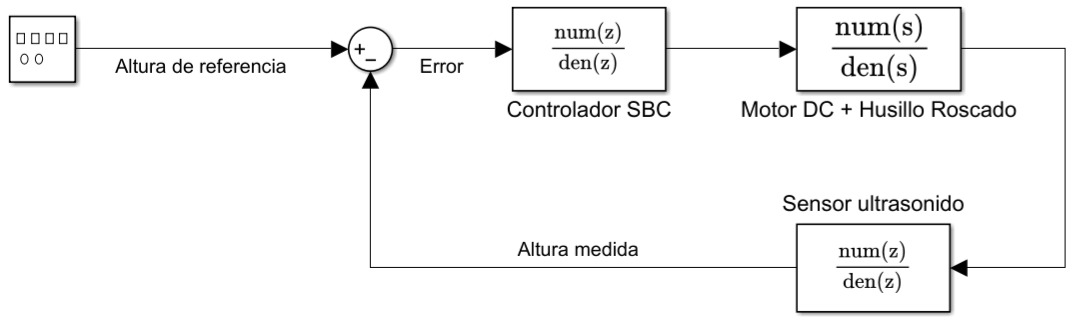
\includegraphics[width=\linewidth]{Recursos/Imagenes/ImagenesDisenoProgramacion/LazoControlAltura.jpg}
	\end{minipage}\hfill
	\begin{minipage}{0.5\textwidth}
		\centering
		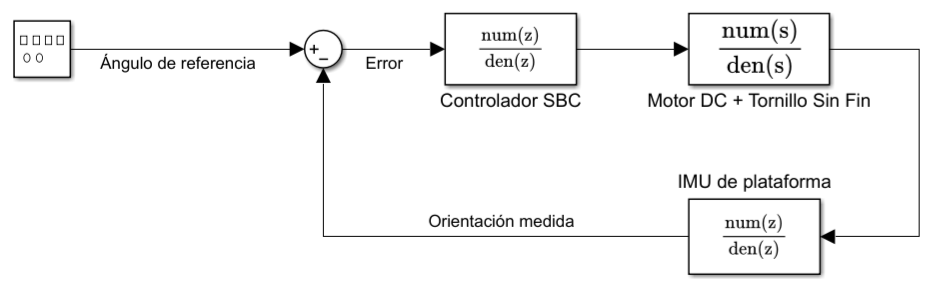
\includegraphics[width=\linewidth]{Recursos/Imagenes/ImagenesDisenoProgramacion/LazoControlAngulo.png}
	\end{minipage}
	\par\medskip
	\raggedright
	\footnotesize \textit{Nota.} Elaboración propia.
	\label{fig:LazosControl}
\end{figure}

%----------------------------------------------------------------------------------------
%	VARIABLES DE CONTROL
%----------------------------------------------------------------------------------------

\section{Variables de control}

La Tabla \ref{tab:variables_monitoreo_control} reúne las variables que el robot mide o regula, con el dispositivo que las mide o las acciona, su interfaz con el procesador y la acción asociada. Las variables meteorológicas se consultan cada $1\text{ s}$ por Modbus RTU (Sección \ref{subsec:puertos_meteo}), dentro del intervalo de $5\text{ s}$ del requerimiento 7 (Tabla \ref{tab:lista_requerimientos}).

\begin{center}
    \footnotesize
    \begin{xltabular}{\textwidth}{|p{2.8cm}|p{2.6cm}|p{2.4cm}|>{\centering\arraybackslash}p{2.0cm}|>{\raggedright\arraybackslash}X|}
        \caption{Variables por monitorear y controlar\label{tab:variables_monitoreo_control}} \\
        \hline
        \rowcolor[HTML]{D9E1F2}
        \textbf{Variable} & \textbf{Dispositivo} & \textbf{Interfaz} & \textbf{Monitorear / Controlar} & \textbf{Acción} \\ \hline
        \endfirsthead

        \multicolumn{5}{c}%
        {{\bfseries \tablename\ \thetable{} -- Continuación de la página anterior}} \\
        \hline
        \rowcolor[HTML]{D9E1F2}
        \textbf{Variable} & \textbf{Dispositivo} & \textbf{Interfaz} & \textbf{Monitorear / Controlar} & \textbf{Acción} \\ \hline
        \endhead

        \hline
        \endfoot

        \hline
        \endlastfoot

        Irradiancia en el plano de los módulos & Piranómetro & RS-485, Modbus RTU & Monitorear & Registro y envío en la trama de telemetría. \\ \hline
        Temperatura y humedad relativa & Sonda de temperatura y humedad & RS-485, Modbus RTU & Monitorear & Registro y envío en la trama de telemetría. \\ \hline
        Velocidad y dirección del viento & Sensor de viento & RS-485, Modbus RTU & Monitorear & Registro, envío de la velocidad en la trama y validación de cada medición según el límite de ráfaga. \\ \hline
        Posición geográfica & Receptor GNSS SAM-M8Q & UART5 de la computadora & Monitorear & Estimación de posición para el Pure Pursuit y envío en la trama. \\ \hline
        Guiñada, cabeceo y alabeo del chasis & BNO055 & I$^2$C del microcontrolador & Monitorear & Rumbo para el Pure Pursuit. \\ \hline
        Velocidad de cada rueda posterior & Encoders E6B2-CWZ6C & Interrupciones externas & Controlar & PID por rueda con la consigna del diferencial electrónico; detección de deslizamiento. \\ \hline
        Ángulo de dirección de cada rueda frontal & Servomotores RDS3225 & PWM a $50\text{ Hz}$ & Controlar & Ángulos de Ackermann; lazo interno de cada servomotor. \\ \hline
        Corriente de cada motor de tracción & Salida CS del controlador de puente H & ADC del microcontrolador & Monitorear & Reducción del ciclo de trabajo sobre $8\text{ A}$. \\ \hline
        Fallas de los controladores de tracción & Salida FLT & Entradas digitales & Monitorear & Detención y reinicio por SLP. \\ \hline
        Ángulo de los brazos de elevación & MPU-6050 del brazo & I$^2$C del microcontrolador & Controlar & Altura del plano óptico; límites de $15^\circ$ a $70.31^\circ$; detección de atascos. \\ \hline
        Alabeo de la plataforma & MPU-6050 del eje basculante & I$^2$C del microcontrolador & Controlar & Inclinación igual a la de los módulos, con tolerancia de $0.5^\circ$. \\ \hline
        Cabeceo de la plataforma & MPU-6050 del eje basculante & I$^2$C del microcontrolador & Monitorear & Verificación de $|p| \leq 1.0^\circ \cdot \tan\beta$ antes de medir. \\ \hline
        Tensión y carga de la batería & Monitor LTC2944 & I$^2$C y salida ALCC & Monitorear & Límite de ciclo de trabajo de tracción; alerta de tensión baja en $21.7\text{ V}$; envío en las banderas de estado. \\ \hline
        Temperatura del gabinete y del chasis & Termistor NTC & ADC del microcontrolador & Monitorear & -- \\ \hline
        Parada de emergencia & Pulsador & Sin procesador & -- & Corta la alimentación de todo el sistema (Sección \ref{subsec:parada_emergencia}). \\ \hline
    \end{xltabular}
\end{center}
% PENDIENTE: acción asociada a la temperatura del termistor y a la alerta de batería (umbral de retorno o de fin de misión); el Capítulo 6 solo define la medición.


\end{document}
